\documentclass[]{article}
\usepackage{lmodern}
\usepackage{amssymb,amsmath}
\usepackage{ifxetex,ifluatex}
\usepackage{fixltx2e} % provides \textsubscript
\ifnum 0\ifxetex 1\fi\ifluatex 1\fi=0 % if pdftex
  \usepackage[T1]{fontenc}
  \usepackage[utf8]{inputenc}
\else % if luatex or xelatex
  \ifxetex
    \usepackage{mathspec}
  \else
    \usepackage{fontspec}
  \fi
  \defaultfontfeatures{Ligatures=TeX,Scale=MatchLowercase}
\fi
% use upquote if available, for straight quotes in verbatim environments
\IfFileExists{upquote.sty}{\usepackage{upquote}}{}
% use microtype if available
\IfFileExists{microtype.sty}{%
\usepackage{microtype}
\UseMicrotypeSet[protrusion]{basicmath} % disable protrusion for tt fonts
}{}
\usepackage[margin=1in]{geometry}
\usepackage{hyperref}
\hypersetup{unicode=true,
            pdftitle={Time Series: Assignment 3},
            pdfauthor={Lucas Cruz Fernandez, 1544674},
            pdfborder={0 0 0},
            breaklinks=true}
\urlstyle{same}  % don't use monospace font for urls
\usepackage{color}
\usepackage{fancyvrb}
\newcommand{\VerbBar}{|}
\newcommand{\VERB}{\Verb[commandchars=\\\{\}]}
\DefineVerbatimEnvironment{Highlighting}{Verbatim}{commandchars=\\\{\}}
% Add ',fontsize=\small' for more characters per line
\usepackage{framed}
\definecolor{shadecolor}{RGB}{248,248,248}
\newenvironment{Shaded}{\begin{snugshade}}{\end{snugshade}}
\newcommand{\AlertTok}[1]{\textcolor[rgb]{0.94,0.16,0.16}{#1}}
\newcommand{\AnnotationTok}[1]{\textcolor[rgb]{0.56,0.35,0.01}{\textbf{\textit{#1}}}}
\newcommand{\AttributeTok}[1]{\textcolor[rgb]{0.77,0.63,0.00}{#1}}
\newcommand{\BaseNTok}[1]{\textcolor[rgb]{0.00,0.00,0.81}{#1}}
\newcommand{\BuiltInTok}[1]{#1}
\newcommand{\CharTok}[1]{\textcolor[rgb]{0.31,0.60,0.02}{#1}}
\newcommand{\CommentTok}[1]{\textcolor[rgb]{0.56,0.35,0.01}{\textit{#1}}}
\newcommand{\CommentVarTok}[1]{\textcolor[rgb]{0.56,0.35,0.01}{\textbf{\textit{#1}}}}
\newcommand{\ConstantTok}[1]{\textcolor[rgb]{0.00,0.00,0.00}{#1}}
\newcommand{\ControlFlowTok}[1]{\textcolor[rgb]{0.13,0.29,0.53}{\textbf{#1}}}
\newcommand{\DataTypeTok}[1]{\textcolor[rgb]{0.13,0.29,0.53}{#1}}
\newcommand{\DecValTok}[1]{\textcolor[rgb]{0.00,0.00,0.81}{#1}}
\newcommand{\DocumentationTok}[1]{\textcolor[rgb]{0.56,0.35,0.01}{\textbf{\textit{#1}}}}
\newcommand{\ErrorTok}[1]{\textcolor[rgb]{0.64,0.00,0.00}{\textbf{#1}}}
\newcommand{\ExtensionTok}[1]{#1}
\newcommand{\FloatTok}[1]{\textcolor[rgb]{0.00,0.00,0.81}{#1}}
\newcommand{\FunctionTok}[1]{\textcolor[rgb]{0.00,0.00,0.00}{#1}}
\newcommand{\ImportTok}[1]{#1}
\newcommand{\InformationTok}[1]{\textcolor[rgb]{0.56,0.35,0.01}{\textbf{\textit{#1}}}}
\newcommand{\KeywordTok}[1]{\textcolor[rgb]{0.13,0.29,0.53}{\textbf{#1}}}
\newcommand{\NormalTok}[1]{#1}
\newcommand{\OperatorTok}[1]{\textcolor[rgb]{0.81,0.36,0.00}{\textbf{#1}}}
\newcommand{\OtherTok}[1]{\textcolor[rgb]{0.56,0.35,0.01}{#1}}
\newcommand{\PreprocessorTok}[1]{\textcolor[rgb]{0.56,0.35,0.01}{\textit{#1}}}
\newcommand{\RegionMarkerTok}[1]{#1}
\newcommand{\SpecialCharTok}[1]{\textcolor[rgb]{0.00,0.00,0.00}{#1}}
\newcommand{\SpecialStringTok}[1]{\textcolor[rgb]{0.31,0.60,0.02}{#1}}
\newcommand{\StringTok}[1]{\textcolor[rgb]{0.31,0.60,0.02}{#1}}
\newcommand{\VariableTok}[1]{\textcolor[rgb]{0.00,0.00,0.00}{#1}}
\newcommand{\VerbatimStringTok}[1]{\textcolor[rgb]{0.31,0.60,0.02}{#1}}
\newcommand{\WarningTok}[1]{\textcolor[rgb]{0.56,0.35,0.01}{\textbf{\textit{#1}}}}
\usepackage{graphicx,grffile}
\makeatletter
\def\maxwidth{\ifdim\Gin@nat@width>\linewidth\linewidth\else\Gin@nat@width\fi}
\def\maxheight{\ifdim\Gin@nat@height>\textheight\textheight\else\Gin@nat@height\fi}
\makeatother
% Scale images if necessary, so that they will not overflow the page
% margins by default, and it is still possible to overwrite the defaults
% using explicit options in \includegraphics[width, height, ...]{}
\setkeys{Gin}{width=\maxwidth,height=\maxheight,keepaspectratio}
\IfFileExists{parskip.sty}{%
\usepackage{parskip}
}{% else
\setlength{\parindent}{0pt}
\setlength{\parskip}{6pt plus 2pt minus 1pt}
}
\setlength{\emergencystretch}{3em}  % prevent overfull lines
\providecommand{\tightlist}{%
  \setlength{\itemsep}{0pt}\setlength{\parskip}{0pt}}
\setcounter{secnumdepth}{0}
% Redefines (sub)paragraphs to behave more like sections
\ifx\paragraph\undefined\else
\let\oldparagraph\paragraph
\renewcommand{\paragraph}[1]{\oldparagraph{#1}\mbox{}}
\fi
\ifx\subparagraph\undefined\else
\let\oldsubparagraph\subparagraph
\renewcommand{\subparagraph}[1]{\oldsubparagraph{#1}\mbox{}}
\fi

%%% Use protect on footnotes to avoid problems with footnotes in titles
\let\rmarkdownfootnote\footnote%
\def\footnote{\protect\rmarkdownfootnote}

%%% Change title format to be more compact
\usepackage{titling}

% Create subtitle command for use in maketitle
\providecommand{\subtitle}[1]{
  \posttitle{
    \begin{center}\large#1\end{center}
    }
}

\setlength{\droptitle}{-2em}

  \title{Time Series: Assignment 3}
    \pretitle{\vspace{\droptitle}\centering\huge}
  \posttitle{\par}
    \author{Lucas Cruz Fernandez, 1544674}
    \preauthor{\centering\large\emph}
  \postauthor{\par}
    \date{}
    \predate{}\postdate{}
  

\begin{document}
\maketitle

\hypertarget{q6}{%
\subsection{Q6}\label{q6}}

We read in the given data as a csv file, which we transformed beforehand
and get the raw gdp data. This will be declared as a time series of
quarterly data with start in 1991 and end in 2017.

\begin{Shaded}
\begin{Highlighting}[]
\NormalTok{gdp_seas_adj <-}\StringTok{ }\KeywordTok{read.csv}\NormalTok{(}\StringTok{"C:/Users/lucas/OneDrive/Dokumente/2. Semester/Time Series/Data/GDP_DE_seas_adj_Fed_StLouis.csv"}\NormalTok{, }\DataTypeTok{sep =} \StringTok{";"}\NormalTok{)}
\NormalTok{gdp <-}\StringTok{ }\NormalTok{gdp_seas_adj[}\DecValTok{2}\NormalTok{]}
\NormalTok{gdp <-}\StringTok{ }\KeywordTok{ts}\NormalTok{(gdp, }\DataTypeTok{frequency =} \DecValTok{4}\NormalTok{, }\DataTypeTok{start =} \KeywordTok{c}\NormalTok{(}\DecValTok{1991}\NormalTok{, }\DecValTok{1}\NormalTok{))}
\end{Highlighting}
\end{Shaded}

We compute the quarterly growth rate as given in the assignment using
R's built-in log and lag functions.

\begin{Shaded}
\begin{Highlighting}[]
\NormalTok{growth_rate <-}\StringTok{ }\KeywordTok{log}\NormalTok{(gdp) }\OperatorTok{-}\StringTok{ }\KeywordTok{log}\NormalTok{(}\KeywordTok{lag}\NormalTok{(gdp))}
\end{Highlighting}
\end{Shaded}

With the data now ready, we can now turn to fitting the ARMA model. We
will use a nested for loop, looping over all combinations of the
respective levels of \(p\) and \(q\), to find the optimal model. We
create an empty matrix that will be filled with the parameters \(p\) and
\(q\) and the respective AIC of the ARMA(p, q) model. The maximum value
of \(p\) and \(q\) we investigate is 3 respectively.

\begin{Shaded}
\begin{Highlighting}[]
\NormalTok{p_max =}\StringTok{ }\DecValTok{3}
\NormalTok{q_max =}\StringTok{ }\DecValTok{3}
\NormalTok{ARMA_models <-}\StringTok{ }\KeywordTok{matrix}\NormalTok{(}\OtherTok{NA}\NormalTok{, }\DataTypeTok{nrow =}\NormalTok{ (p_max }\OperatorTok{+}\StringTok{ }\DecValTok{1}\NormalTok{)}\OperatorTok{*}\NormalTok{(q_max }\OperatorTok{+}\StringTok{ }\DecValTok{1}\NormalTok{), }\DataTypeTok{ncol =} \DecValTok{3}\NormalTok{)}
\KeywordTok{colnames}\NormalTok{(ARMA_models) <-}\StringTok{ }\KeywordTok{c}\NormalTok{(}\StringTok{"p"}\NormalTok{, }\StringTok{"q"}\NormalTok{, }\StringTok{"AIC"}\NormalTok{)}
\CommentTok{#loop over p }
\NormalTok{count <-}\StringTok{ }\DecValTok{0}
\ControlFlowTok{for}\NormalTok{(p }\ControlFlowTok{in} \DecValTok{0}\OperatorTok{:}\DecValTok{3}\NormalTok{)\{}
  \CommentTok{#loop over q }
    \ControlFlowTok{for}\NormalTok{(q }\ControlFlowTok{in} \DecValTok{0}\OperatorTok{:}\DecValTok{3}\NormalTok{)\{}
\NormalTok{      count <-}\StringTok{ }\NormalTok{count }\OperatorTok{+}\StringTok{ }\DecValTok{1}
\NormalTok{      ARMA_models[count, }\DecValTok{1}\NormalTok{] <-}\StringTok{ }\NormalTok{p }
\NormalTok{      ARMA_models[count, }\DecValTok{2}\NormalTok{] <-}\StringTok{ }\NormalTok{q}
\NormalTok{      model <-}\StringTok{ }\KeywordTok{arima}\NormalTok{(}\DataTypeTok{x =}\NormalTok{ growth_rate, }\DataTypeTok{order =} \KeywordTok{c}\NormalTok{(p, }\DecValTok{0}\NormalTok{ , q))}
\NormalTok{      ARMA_models[count, }\DecValTok{3}\NormalTok{] <-}\StringTok{ }\NormalTok{model}\OperatorTok{$}\NormalTok{aic }
\NormalTok{    \}}
\NormalTok{\}}
\end{Highlighting}
\end{Shaded}

Now that we calculated the AIC for each model we can simply get model
with the lowest AIC.

\begin{Shaded}
\begin{Highlighting}[]
\NormalTok{p_opt <-}\StringTok{ }\NormalTok{ARMA_models[}\KeywordTok{which}\NormalTok{(ARMA_models[, }\DecValTok{3}\NormalTok{] }\OperatorTok{==}\StringTok{ }\KeywordTok{min}\NormalTok{(ARMA_models[, }\DecValTok{3}\NormalTok{])), }\DecValTok{1}\NormalTok{]}
\NormalTok{q_opt <-}\StringTok{ }\NormalTok{ARMA_models[}\KeywordTok{which}\NormalTok{(ARMA_models[, }\DecValTok{3}\NormalTok{] }\OperatorTok{==}\StringTok{ }\KeywordTok{min}\NormalTok{(ARMA_models[, }\DecValTok{3}\NormalTok{])), }\DecValTok{2}\NormalTok{]}
\NormalTok{AIC_opt <-}\StringTok{ }\NormalTok{ARMA_models[}\KeywordTok{which}\NormalTok{(ARMA_models[, }\DecValTok{3}\NormalTok{] }\OperatorTok{==}\StringTok{ }\KeywordTok{min}\NormalTok{(ARMA_models[, }\DecValTok{3}\NormalTok{])), }\DecValTok{3}\NormalTok{]}
\end{Highlighting}
\end{Shaded}

We can see that \$p = \$ 1 and \$q = \$0, which has an AIC of \$AIC = \$
-726.9300683. The model with the best fit using the AIC as the
evaluation criterion is therefore an ARMA(1, 0) model. The coefficients
of this specification are then:

\begin{Shaded}
\begin{Highlighting}[]
\NormalTok{ARMA_opt <-}\StringTok{ }\KeywordTok{arima}\NormalTok{(}\DataTypeTok{x =}\NormalTok{ growth_rate, }\DataTypeTok{order =} \KeywordTok{c}\NormalTok{(p_opt, }\DecValTok{0}\NormalTok{, q_opt))}
\NormalTok{ARMA_opt}\OperatorTok{$}\NormalTok{coef}
\end{Highlighting}
\end{Shaded}

\begin{verbatim}
##          ar1    intercept 
##  0.269877617 -0.007158814
\end{verbatim}

To evaluate whether it captures all dynamics we can take a look at the
autcorrelation between the residuals of our optimal model.

\begin{Shaded}
\begin{Highlighting}[]
\CommentTok{#estimate the optimal model to get the residuals}
\NormalTok{res <-}\StringTok{ }\KeywordTok{residuals}\NormalTok{(ARMA_opt)}
\NormalTok{autocorr <-}\StringTok{ }\KeywordTok{acf}\NormalTok{(res)}
\end{Highlighting}
\end{Shaded}

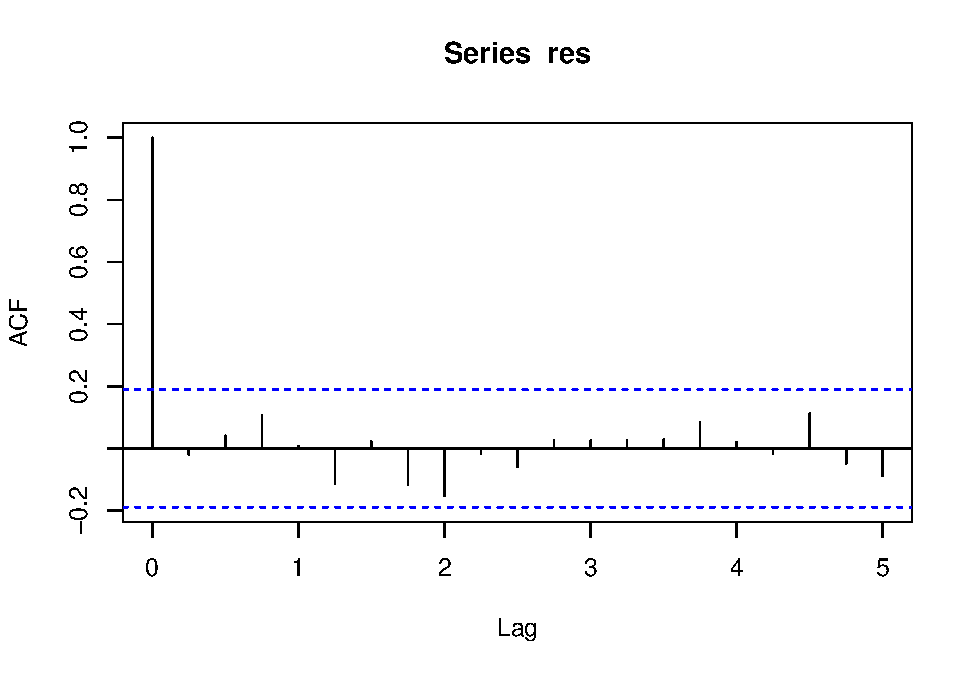
\includegraphics{figure-latex/unnamed-chunk-7-1.pdf}

We can clearly see that after the current period (i.e.~\(h > 0\)) there
is no significant autocorrelation between the residuals further
strengthening the result of our model evaluation based on the AIC.


\end{document}
